\section{Results}

\begin{figure}[ht]
\centering
\begin{tabular}{| l | l | c |}
  \hline
  ID & Description & Link \\
  \hline
  1 & Single Agent Results, coloured by opposite surface& \href{https://barrett370.github.io/Y4-Diss/single-agent-result-1404-col}{url} \\
  2 & Multi agent results & \href{https://barrett370.github.io/Y4-Diss/multi-agent-result-1304}{url} \\
  3 & Multi agent results, coloured by opposite surface & \href{https://barrett370.github.io/Y4-Diss/multi-agent-result-1904-col}{url} \\
  4 & Multi agent results, coloured by opposite surface, fitness threshold = 40 & \href{https://barrett370.github.io/Y4-Diss/multi-agent-result-1304-lim40-col}{url} \\
  5 & Multi agent results, with fitness-planning time overlayed, fitness threshold=100 & \href{https://barrett370.github.io/Y4-Diss/multi-agent-result-shared-lim100}{url} \\


  \hline
\end{tabular}
\caption{\label{tab:plotlinks} External links to dynamic plots}
\end{figure}

Due to the high dimensionality of my search space, I cannot visualise the objective function of my GA.

\begin{figure}[ht]
  \centering
  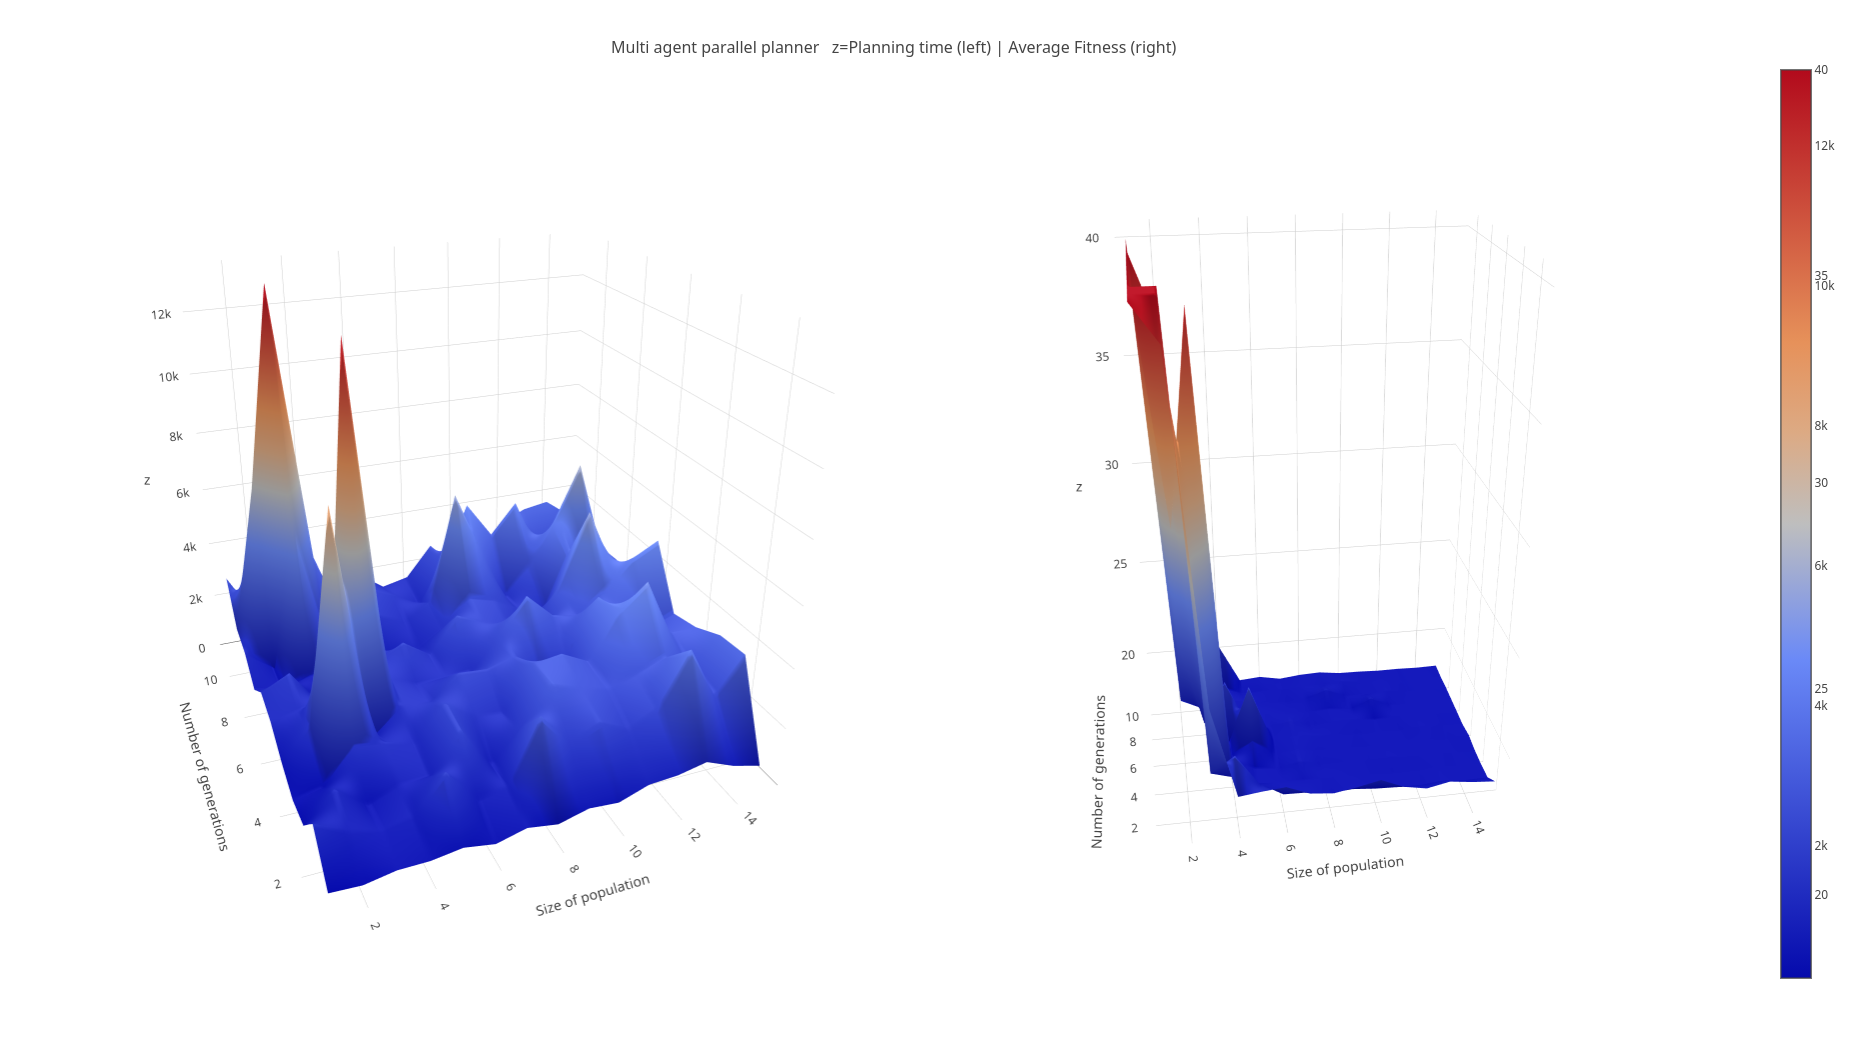
\includegraphics[scale=0.19]{figures/ma-1304-lim40.png}
  \caption{\label{fig:ma-lim40} Multi agent planning number of generations against size of population against planning time (left), fitness limited at 40 (right)}
\end{figure}
\todo{Check units for planning time + add link to hosted dynamic version}

\begin{figure}[ht]
  \centering
  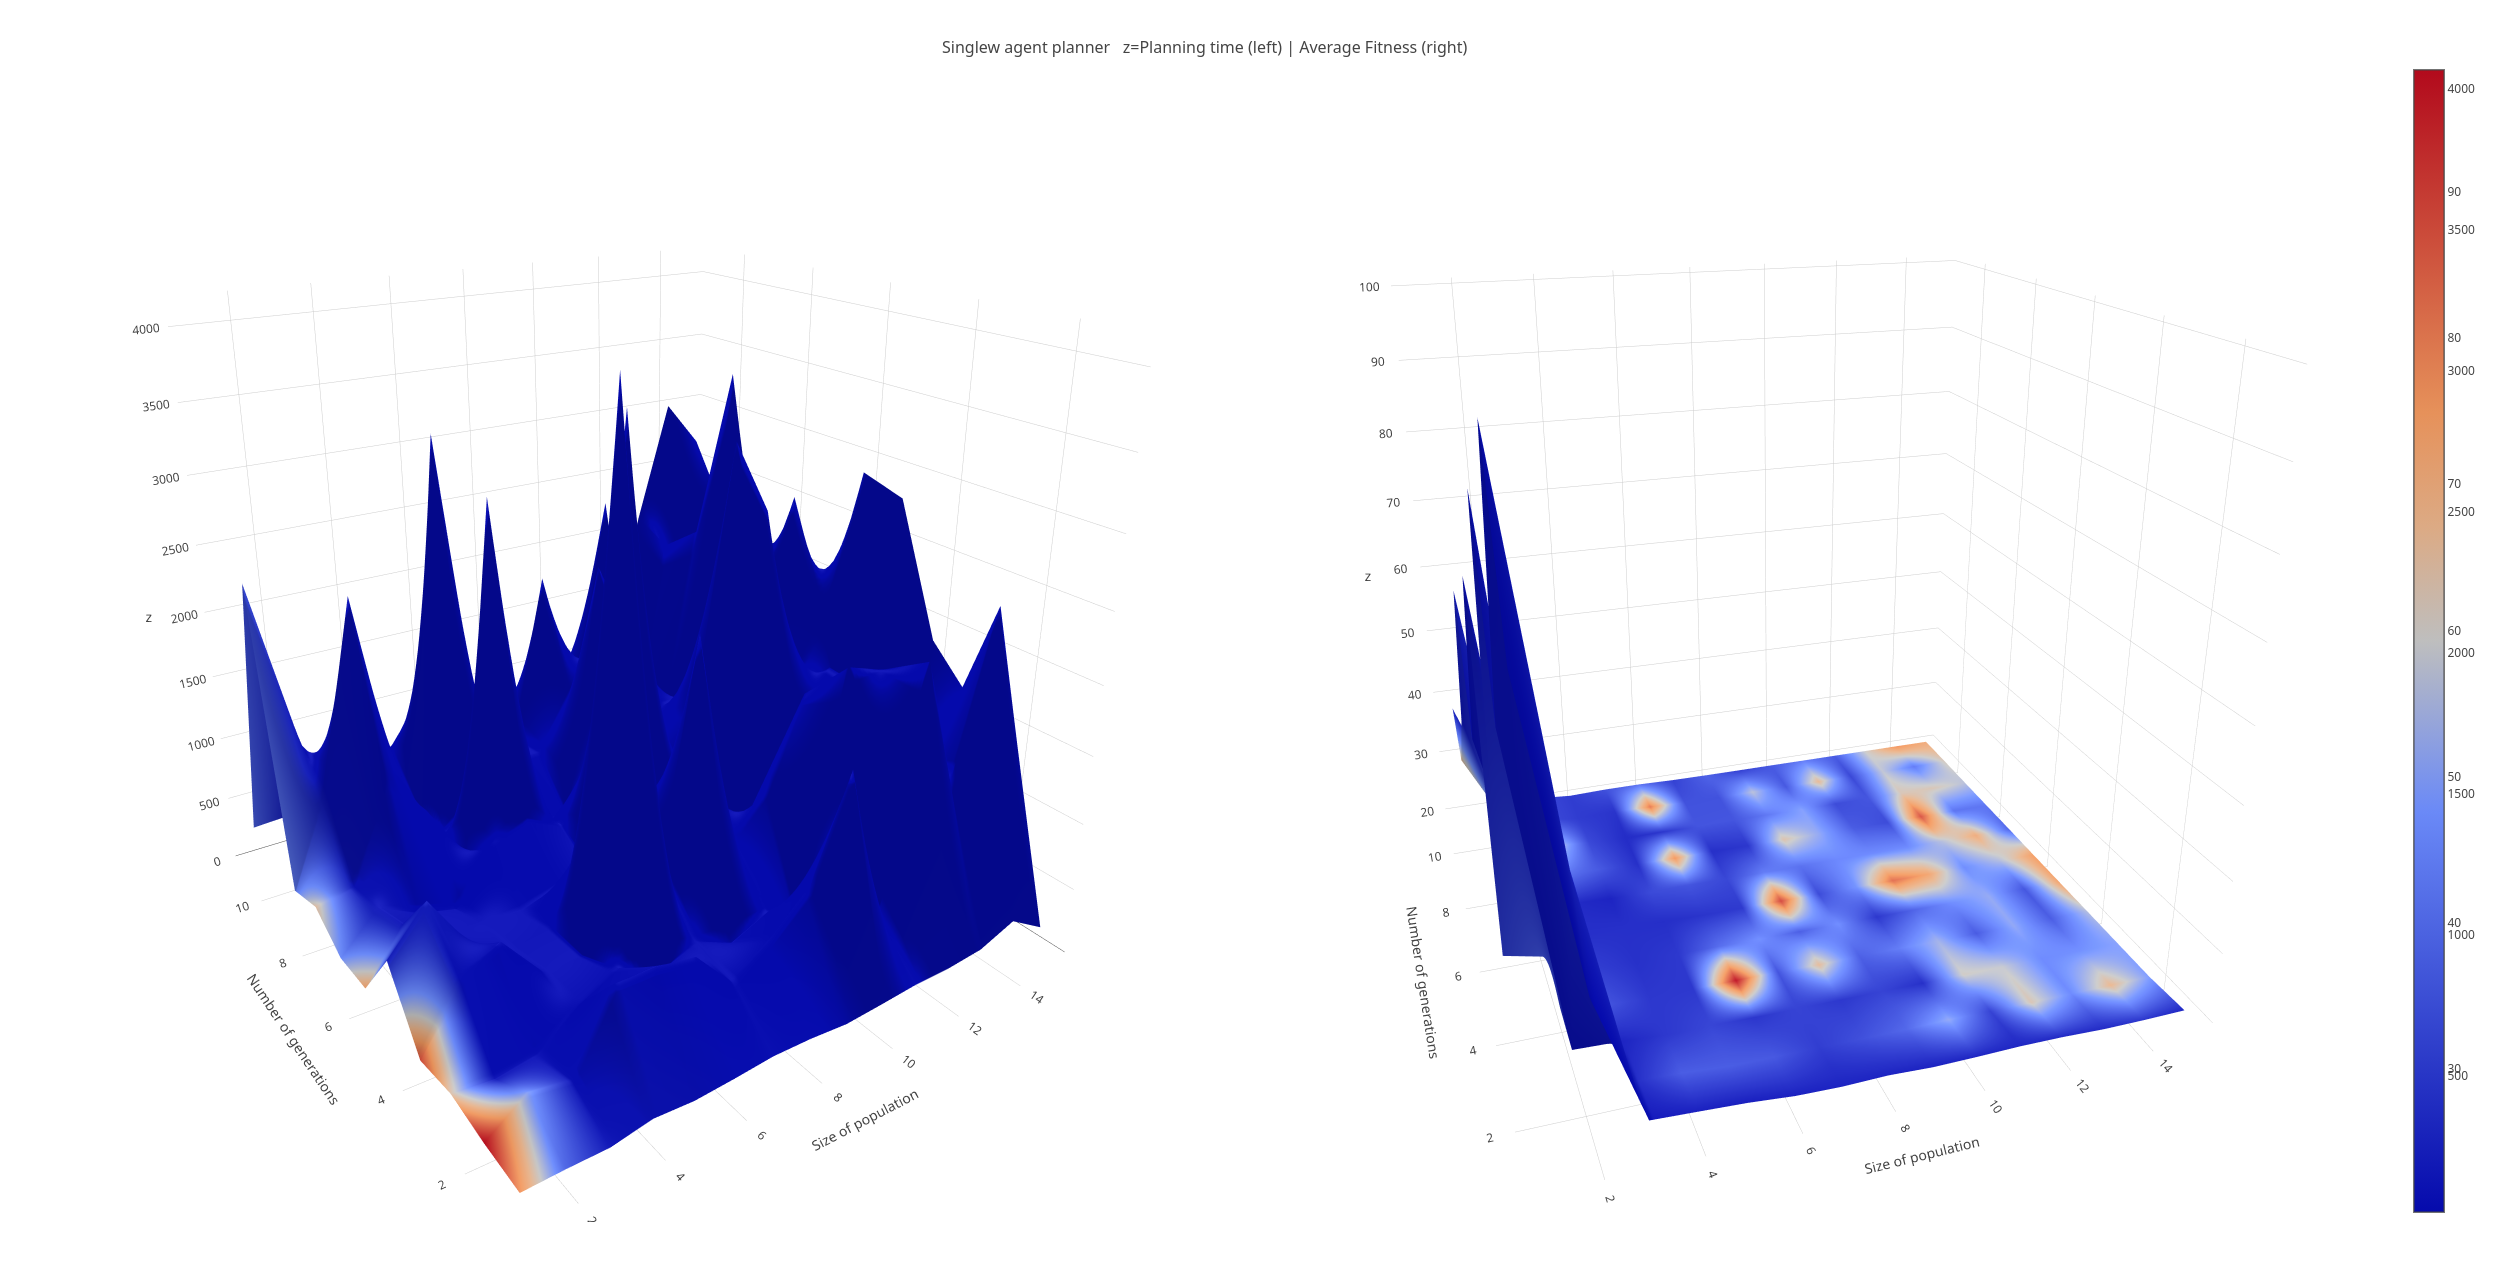
\includegraphics[scale=0.14]{figures/sa-1404-col.png}
  \caption{\label{fig:sa-col} Single agent planning: number of generations against size of population against planning time (left), fitness (right)}
\end{figure}
\todo{Check units for planning time + add link to hosted dynamic version}

My results were achieved by
\subsection{Bézier Curves}
\todo[inline]{expand on this section, talk about issues of finding intersection, possible GPU applications}

Bézier curves have been utilised in this project to encode and represent the route of a vehicle. As mentioned in Section~\ref{sec:back-bezier-curves}, there are many reasons I originally selected them for this task. However, over the course of implementation and testing, a number of downsides have been presented.

\subsection{Cooperative Planning}
\label{subsec:eval-cooperativeplanning}

My solution to the problem of planning $n$ non-colliding routes for $n$ agents was so wrap my existing \texttt{GA} function in a cooperative \textit{layer}. This cooperative layer relied on a function for detecting collisions which had extremely high overhead, at one point causing around 50x slowdown in the running time of the function. Detecting intersections between two Bézier curves is a non-trivial task with the best methods taking the same approach of recursive subdivision that I utilised.

\todo[inline]{make mention of possible GPU implementations such at in~\cite{robergeFastGeneticAlgorithm2018}, modern enterprise GPUs have around 4000-10000 cores, approximately the max number of curve splits and comparisons in a binary check of depth 6. Being able to do this in a single cycle would result in a huge speedup, paper uses Titan X }



%TC:macro \todo 1


%%% Local Variables:
%%% mode: latex
%%% TeX-master: "report"
%%% End:
